\newpage
\hypertarget{treeToModel vis}{}
\subsection{The visual transformation rules}
\visHeader

Some sort of content to keep from jumping immediately into an item. We need to break it down, we want to separate multiple instances. Remember -- they follow a
precondition/postcondition format\ldots While it may seem like there are a lot of rules, you'll notice that they are all neccessary and make the transformation
both easy to execute and understand.

\begin{itemize}

\subsubsection{FolderToLibraryRule} % ---------------------------------

\item[$\blacktriangleright$] Expand the \texttt{<<Rules Package>>} node in EA and open the \texttt{Rules} diagram. Create a new rule named
\texttt{FolderToLibraryRule}, double-clicking the new element to open its diagram. Complete the rule as depicted in Fig.~\ref{ea:FolderIntoLibrary_Complete}.
Remember -- we established that first correspondence type when creating the TGG schema in Section 1.

\vspace{0.5cm}

\begin{figure}[htbp]
\begin{center}
  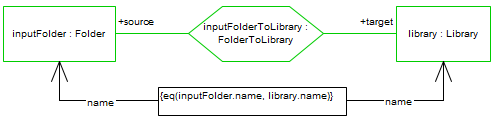
\includegraphics[width=\textwidth]{ea_FolderToLibraryRule}
  \caption{completed folder into library}
  \label{ea:FolderIntoLibrary_Complete}
\end{center}
\end{figure}

\item[$\blacktriangleright$] We're able to use this entire rule as context for the next rule in order to handle the creation of shelves. Select
\texttt{inputFolder}, \texttt{in\-put\-Fol\-der\-To\-Lib\-rary,} and \texttt{library}, then use the eMoflon control panel to \texttt{derive} a new rule. Name
this \texttt{ForAllShelfRule}. % Integrating green with black..

\subsubsection{ForAllShelfRule} % ---------------------------------

\item[$\blacktriangleright$] This will open a new diagram with three black objects, representing the context. This rule is remarkably similar to
\texttt{FolderToLibraryRule}, except it will need two green links connecting the new elements to their respective container. Complete \texttt{ForAllShelfRule}
as depicted in Fig.~\ref{ea:ForAllShelves_Complete}; You'll need to create a new correspondence type in either the schema (as we did
in the beginning) or on-the-fly by selecting \texttt{Create new Link} in the quick-link dialogue.\footnote{see Part, Section \update}

\clearpage

\begin{figure}[htbp]
\begin{center}
  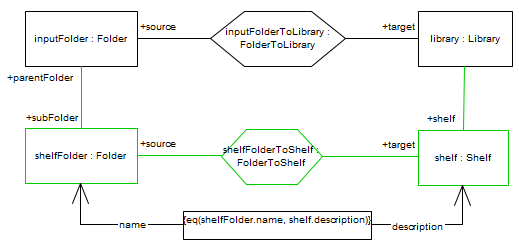
\includegraphics[width=0.8\textwidth]{ea_ForAllShelfRule}
  \caption{completed ForAllShelves}
  \label{ea:ForAllShelves_Complete}
\end{center}
\end{figure}

\subsubsection{NodeToDictionaryRule} % ---------------------------------

\item[$\blacktriangleright$] Now we can handle the dictionary \texttt{File} elements. Analogously to how you began the previous rule, select
\texttt{shelfFolder}, \texttt{FolderToShelf}, and \texttt{shelf}, and derive \texttt{NodeToDictionaryRule}.

\item[$\blacktriangleright$] Build it as shown in Fig.~\ref{ea:NodeToDictionary_Complete}. As you can see, this rule creates a consistency between
\texttt{dictionaryNode} and the \texttt{dictionary} instance, and only handles the first \texttt{titleNode} in the tree structure. Nearly every element is
involved in order to correctly set the \texttt{dictionary} and \texttt{dictionaryFile} names in two different constraints!

\begin{figure}[htbp]
\begin{center}
  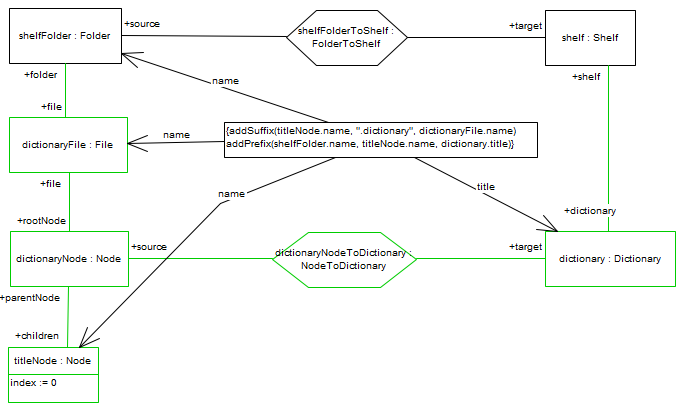
\includegraphics[width=\textwidth]{ea_NodeToDictionaryRule}
  \caption{completed NodeToDictionary}
  \label{ea:NodeToDictionary_Complete}
\end{center}
\end{figure}


\item[$\blacktriangleright$] Please note that the \texttt{index} \emph{attribute constraint} is required in order to ensure that the node with the title
information is correctly matched. We could have also included a \texttt{node} to handle the author, a third, fourth, or even tenth \texttt{node} connected to
\texttt{DictionaryNode}, but that would mean the pattern absolutely has to match to an author and ten elements, which may not always exist. Instead, we'll
create separate rules for each of these types which can be called as many times as necessary.

\subsubsection{ForAllEntryRule} % ---------------------------------

\item[$\blacktriangleright$] Let's handle the \texttt{entry} elements first. Create and complete \texttt{For\-All\-Ent\-ry\-Rule} and depicted in
Fig.~\ref{ea:ForAllEntry_Complete}. We needed to match both a \texttt{contentNode} and \texttt{indexNode} to each \texttt{entryNode}, bound by their
\texttt{index} values in order to ensure the correct EString attributes were set to an \texttt{entry}'s \texttt{content} and \texttt{level} values.

\vspace{0.5cm}

\begin{figure}[htbp]
\begin{center}
  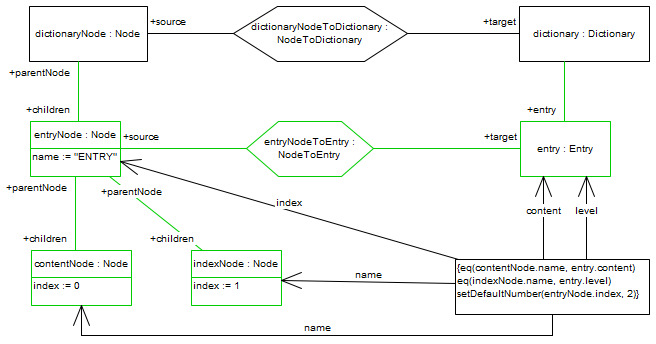
\includegraphics[width=\textwidth]{ea_ForAllEntryRule}
  \caption{completed ForAllEntry}
  \label{ea:ForAllEntry_Complete}
\end{center}
\end{figure}

\clearpage

\item[$\blacktriangleright$] Return to \texttt{NodeToDictionaryRule}. We need to think about what context elements we'll need for our next rule to handle
authors. Not only will we need \texttt{DictionaryNode} and \texttt{dictionary} as we did in \texttt{ForAllEntry}, we'll also need \texttt{shelf} and
\texttt{library} in order to satisfy the \texttt{Dictionary} metamodel, where each \texttt{author} is linked to both individual \texttt{dictionary} and
\texttt{library} elements. Derive and create \texttt{AuthorRule} as depicted below Fig.~\ref{ea:AuthorRule}

\subsubsection{AuthorRule} % ---------------------------------

\begin{figure}[htbp]
\begin{center}
  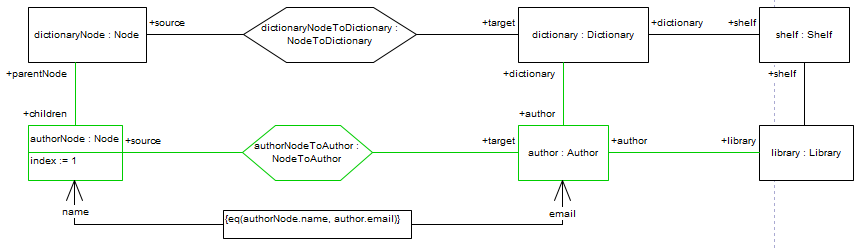
\includegraphics[width=\textwidth]{ea_AuthorRule}
  \caption{completed AuthorRule}
  \label{ea:AuthorRule}
\end{center}
\end{figure}

\end{itemize}

There is another part of handling authors when transforming from our tree to our instance model. Right now, we have specified that
for every \texttt{authorNode} the rule finds, create an \texttt{author} instance. This would be fine if we had unique authors for \emph{every} dictionary
\texttt{File}, but look at both of the french \texttt{numbers} files -- they both have the same contact information. This means that our \texttt{Dictionary}
will have two identical author instances for one Library. 

Some users may be okay with this, and not care about multiples, so long as all the correct information is there, while others would prefer a minimalist
structure. How can we refine this rule so that the user can quickly implement one or othe other?

eMolfon's visual syntax has a cool \emph{refinement} feature which enables you to adjust specific elements in a rule. This is exactly what we're looking for --
our rules to handle either creating or checking for an existing author are nearly \emph{identical} to \texttt{AuthorRule}, save for the binding (and therefore
reference links) on \texttt{authorNode}.

\begin{itemize}

\item[$\blacktriangleright$] Return to the \texttt{Rules} diagram. Since we're no longer looking to implement \texttt{AuthorRule} directly, we need to update
its definition to an \texttt{abstract} class. Select the rule, then hit \texttt{alt + enter} top open its properties dialogue.

\item[$\blacktriangleright$] Switch to the \texttt{details} tab, and select \texttt{Abstract} from the list of class types (Fig.~\ref{ea:abstractDetails}). 
Affirm and close by pressing \texttt{Ok}.

\begin{figure}[htbp]
\begin{center}
  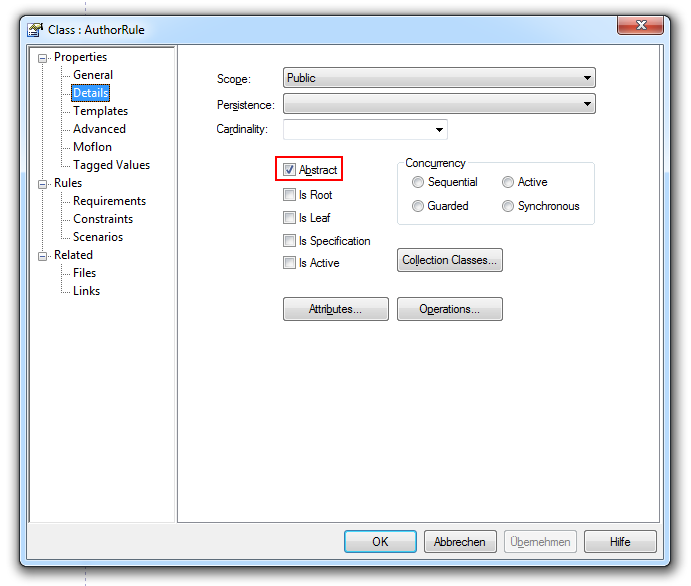
\includegraphics[width=\textwidth]{ea_abstractDetails}
  \caption{completed AuthorRule}
  \label{ea:abstractDetails}
\end{center}
\end{figure}

\end{itemize}

Now to develop our two rules. The key idea when building refinements is to imagine the rules are being placed directly over the
pattern they inherit from, similar to a transparency sheet. Theses rules will execute \texttt{AuthorRule} exactly, except for whatever modficiations you make.

Let's create the rule to handle an already existing author first. Inspecting \texttt{AuthorRule}, we still want the rule to match a new \texttt{authorNode}
and create a link between \texttt{author} and \texttt{dictionary}, but the link between \texttt{author} variable and the link connecting it to \texttt{library}
should already exist, i.e., be 'black.'

\begin{itemize}

\subsubsection{ExistingAuthorRule} % ---------------------------------

\item[$\blacktriangleright$] In \texttt{AuthorRule}'s diagram, select \texttt{authorNode} and \texttt{library}, and under the ``eMoflon TGG Functions'' tab in
the eMoflon control panel, press \texttt{Derive}. 

\item[$\blacktriangleright$] Enter \texttt{ExistingAuthorRule} as the rule's name but, given that we're just wanting to replace the selected elements, and not
use them as context elements, be sure to select the exact copy option (Fig.~\ref{ea:deriveRefinement}).

\begin{figure}[htbp]
\begin{center}
  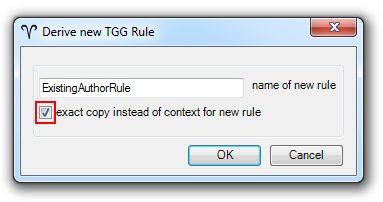
\includegraphics[width=0.6\textwidth]{ea_deriveRefinement}
  \caption{completed AuthorRule}
  \label{ea:deriveRefinement}
\end{center}
\end{figure}

\item[$\blacktriangleright$] The rule diagram will open in the editor, with the elements in the same place you copied them from. You can move the model around
if the white space is bothering you, but the ``transparency'' will  be much easier to visualise if you leave it as-is.

\item[$\blacktriangleright$] Change the 'green' binding operator on \texttt{author} and the link to \texttt{Check Only}. That's everything!

\subsubsection{NewAuthorRule} % ---------------------------------

\item[$\blacktriangleright$] Return to \texttt{AuthorRule}. For reasons that will be explained shortly in the next section, derive a copy of \texttt{authorNode}
and \texttt{library}. Don't modify either variable -- since we have now defined \texttt{AuthorRule} as an abstract class, it needs a concrete rule to execute
it.

\item[$\blacktriangleright$] Open the \texttt{Rule} diagram one last time. We need the new rules to inherit from the \texttt{AuthorRule}. Quick-link
each to the root rule, choosing \texttt{Create Refinement Link} from the context menu. Your diagram should now resemble Fig.~\ref{ea:refinementClasses}.

\begin{figure}[htbp]
\begin{center}
  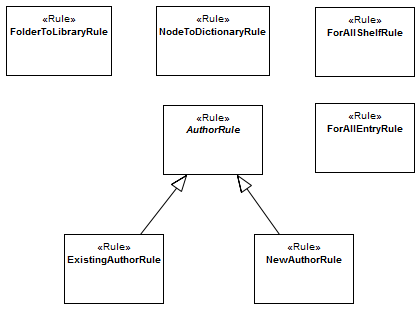
\includegraphics[width=0.6\textwidth]{ea_refinementLinks}
  \caption{Finished \texttt{Rules} diagram}
  \label{ea:refinementClasses}
\end{center}
\end{figure}


\item[$\blacktriangleright$] You're nearly done! Make sure everything is saved, and validate your TGG. If a dialogue appears saying the attempt was
unsuccessful, you may simply need to update the schema diagram which may not contain the new correspondence types you created on the fly. To do so, open
\texttt{dictionaryCodeAdapter}, right click anywhere in the diagram and add any missing elements by navigating to ``Insert Existing Element''
(Fig.~\ref{ea:insertContext}), and selecting the missing correspondence types from the root package's tree (Fig.~\ref{ea:insertTree}).

\begin{figure}[htbp]
   \centering
      \subfloat[Right-click to open the context menu]{
        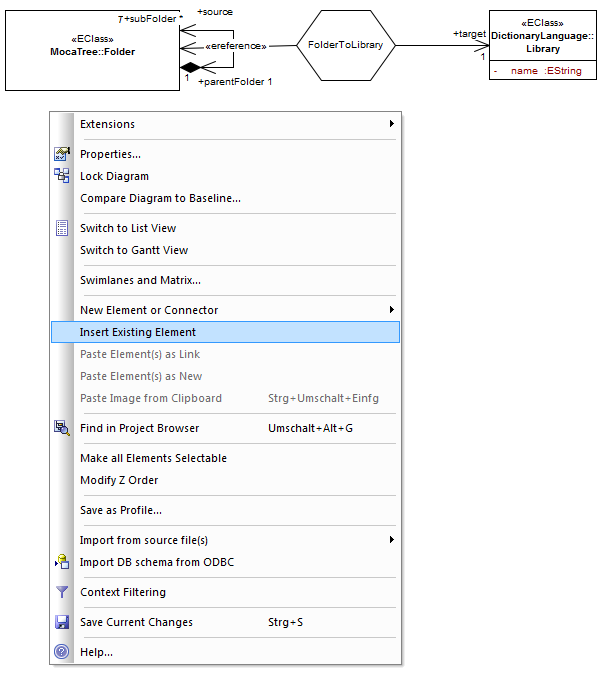
\includegraphics[width=0.7\textwidth]{ea_InsertExistingElements}
        \label{ea:insertContext}
      }
      \\
      \subfloat[Check your \texttt{TGG}, \texttt{DictionaryLanguage}, and \texttt{MocaTree} packages]{
        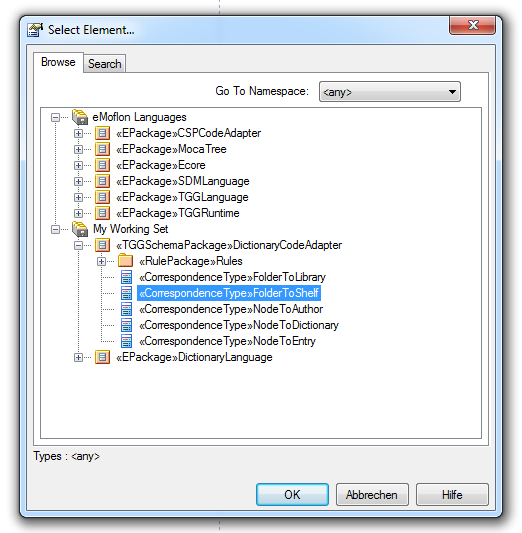
\includegraphics[width=0.7\textwidth]{ea_insertElementTree}
        \label{ea:insertTree}
      }
      % \caption{Updating your schema with missing elements}
\end{figure}

\item[$\blacktriangleright$] Your schema diagram should resemble Fig.~\ref{ea:Schema_Complete} upon exit. Validate the project once again, then switch to the
Eclipse workspace and refresh the package explorer to generate new code. Great work!

\newpage

\vspace*{3cm}

\begin{figure}[htbp]
\begin{center}
  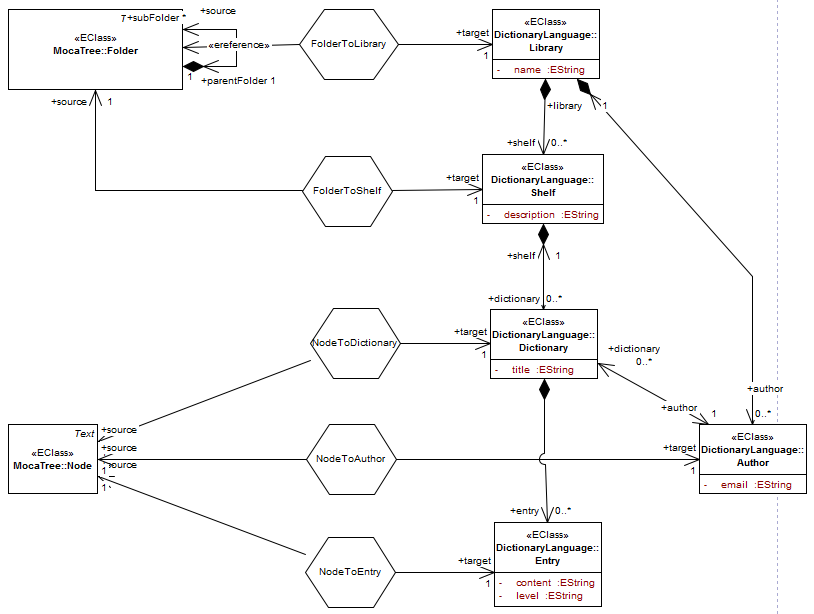
\includegraphics[width=\textwidth]{ea_finalSchema}
  \caption{Completed TGG schema diagrams}
  \label{ea:Schema_Complete}
\end{center}
\end{figure}

\jumpSingle{t2m close}

\end{itemize}
